\documentclass[a4]{scrartcl}

% \usepackage[ngerman]{babel}
\usepackage[utf8]{inputenc}
\usepackage{mathtools}
\usepackage{amsmath}
\usepackage{amssymb}
\usepackage{geometry}
\usepackage{scrlayer-scrpage}
\usepackage{float}
\usepackage{xcolor}
\pagestyle{scrheadings}
\clearscrheadfoot

\usepackage[backend=biber, maxbibnames=99]{biblatex}
\addbibresource{references.bib}

\setlength{\parindent}{0cm}


\geometry{
  paper=a4paper, % Change to letterpaper for US letter
  top=2cm, % Top margin
  bottom=1.5cm, % Bottom margin
  left=2cm, % Left margin
  right=3cm, % Right margin
}

\ohead{\\
Pina Kolling\\
piko0011}

\usepackage[framemethod=TikZ]{mdframed}

% Style %
\mdfdefinestyle{enviStyle}{
   innertopmargin = 10pt,
  linewidth      = 1pt,
  frametitlerule = true,
  roundcorner    = 2pt%
}


\newenvironment{CountingDefinition}[2][]{%
   \ifstrempty{#1}%
   {\mdfsetup{%
      frametitle={{\strut ~}}}
   }%
   {\mdfsetup{%
      frametitle={{\strut ~#1}}}%
   }%
   \mdfsetup{
      nobreak                   = true,
     linecolor                 = gray,
    frametitlebackgroundcolor = gray!50,
    style                     = enviStyle
   }
   \begin{mdframed}[]\relax%
   \label{#2}}{\end{mdframed}}

\begin{document}

\section*{Summary: Lecture 10}

Summary for the chapters \textit{11.1} up to page 245 and \textit{11.2} (page 258 optional). \cite{book, CC}

\begin{CountingDefinition}[Randomized algorithms]{def:validLabelPlacement}
Algorithms based on randomization.


(The algorithm employs a degree of randomness as part of its logic or procedure.)
\end{CountingDefinition}

\subsection*{Symbolic Determinants}

\begin{CountingDefinition}[Bipartite Graph]{def:validLabelPlacement}
A graph $G = (U,V,E)$ is called bipartite if the vertices can be divided into two disjoint and independent sets $U$ and $V$. (There are no edges between two elements of $U$ or two elements of $V$).

\begin{figure}[H]
\begin{center}
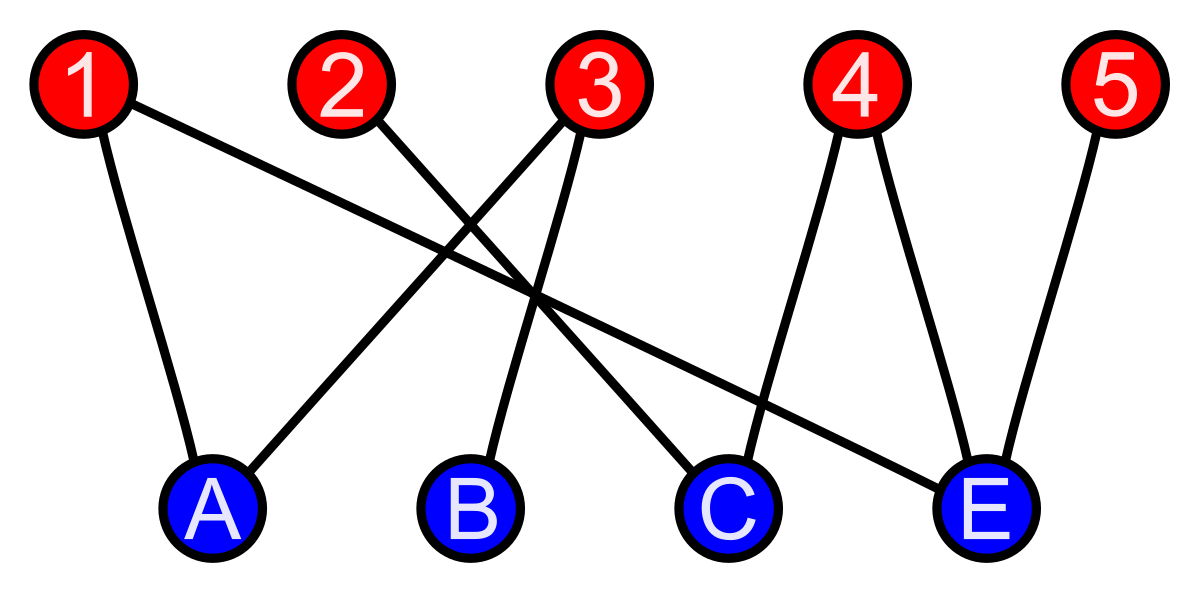
\includegraphics[scale=0.13]{bg1.png}
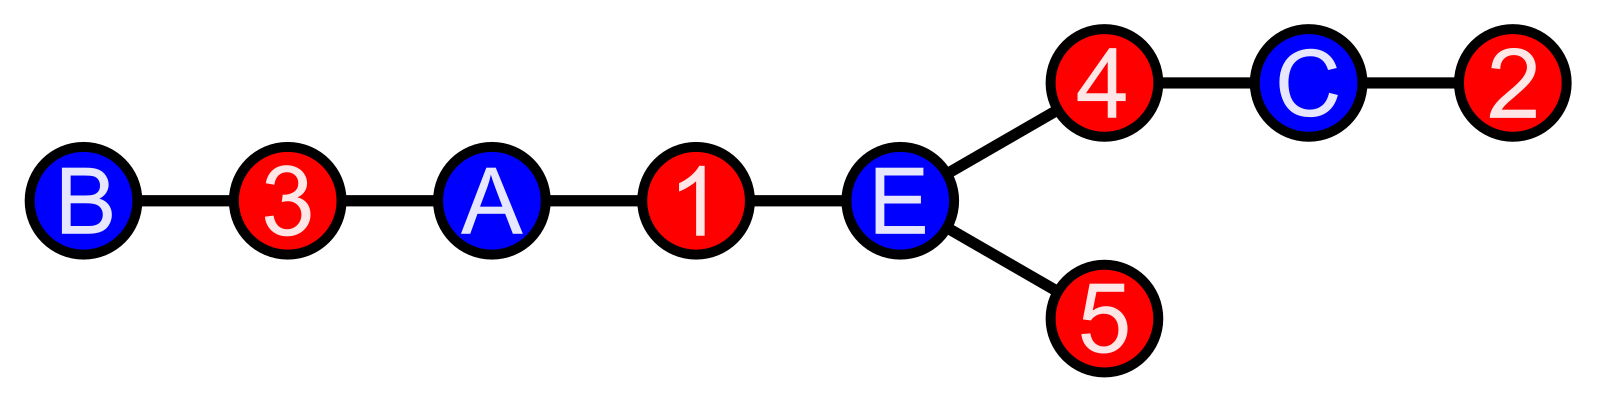
\includegraphics[scale=0.13]{bg2.png}
\end{center}
\caption{Examples of bipartife graphs with $U$ and $V$ marked in red and blue \cite{bg}}
\end{figure}

\end{CountingDefinition}

\begin{CountingDefinition}[Problem: BipartiteMatching]{def:validLabelPlacement}
asdf
\end{CountingDefinition}

\begin{itemize}
\item
\end{itemize}

\color{red} TODO \\
\color{black}
\color{violet} Questions:
\color{black}

\begin{itemize}
\item some slides about stuff that is not in the book
\item Satz von Rice
\end{itemize}


\newpage

\printbibliography




\end{document}